% XeLaTeX can use any Mac OS X font. See the setromanfont command below.
% Input to XeLaTeX is full Unicode, so Unicode characters can be typed directly into the source.

% The next lines tell TeXShop to typeset with xelatex, and to open and save the source with Unicode encoding.

%!TEX TS-program = xelatex
%!TEX encoding = UTF-8 Unicode

\documentclass[12pt]{article}
\usepackage{geometry}                % See geometry.pdf to learn the layout options. There are lots.
\geometry{letterpaper}                   % ... or a4paper or a5paper or ... 
%\geometry{landscape}                % Activate for for rotated page geometry
%\usepackage[parfill]{parskip}    % Activate to begin paragraphs with an empty line rather than an indent
\usepackage{graphicx}
\usepackage{amssymb}
\usepackage[slantfont,boldfont]{xeCJK}
\usepackage{booktabs}
\usepackage{bm}
\usepackage{float}

% Will Robertson's fontspec.sty can be used to simplify font choices.
% To experiment, open /Applications/Font Book to examine the fonts provided on Mac OS X,
% and change "Hoefler Text" to any of these choices.

\usepackage{fontspec,xltxtra,xunicode}
\defaultfontfeatures{Mapping=tex-text}
\setromanfont[Mapping=tex-text]{Hoefler Text}
\setsansfont[Scale=MatchLowercase,Mapping=tex-text]{Gill Sans}
\setmonofont[Scale=MatchLowercase]{Andale Mono}
\usepackage{indentfirst} 
\usepackage{amsmath}
\setlength{\parindent}{2em}
\usepackage{listings}
\usepackage[usenames,dvipsnames]{xcolor}
\definecolor{mygreen}{rgb}{0,0.6,0}
\definecolor{mygray}{rgb}{0.5,0.5,0.5}
\definecolor{mymauve}{rgb}{0.58,0,0.82}
\lstset{
 backgroundcolor=\color{lightgray}, 
 basicstyle = \footnotesize,       
 breakatwhitespace = false,        
 breaklines = true,                 
 captionpos = b,                    
 commentstyle = \color{mygreen}\bfseries,
 extendedchars = false,             
 frame =shadowbox, 
 framerule=0.5pt,
 keepspaces=true,
 keywordstyle=\color{blue}\bfseries, % keyword style
 language = C++,                     % the language of code
 otherkeywords={string}, 
 numbers=left, 
 numbersep=5pt,
 numberstyle=\tiny\color{mygray},
 rulecolor=\color{black},         
 showspaces=false,  
 showstringspaces=false, 
 showtabs=false,    
 stepnumber=1,         
 stringstyle=\color{mymauve},        % string literal style
 tabsize=2,          
 title=\lstname                      
}

\setmainfont{Times New Roman}

\title{Kalmann Filter程序设计报告}
\author{刘沐林}
%\date{}                                           % Activate to display a given date or no date

\begin{document}
\maketitle

\tableofcontents

\section{背景}

Kalmann Filter是在实际工程应用中常用的状态预测、估计、修正方法, 能够使用观测量和动力学模型对实际的状态量进行修正和预测. 在本工作中, Kalmann滤波被用来预测信号在下一组数据中的状态, 从而便于后续对信号的追踪.

\section{技术参数}

编写语言: C++

标准: C++17

依赖: 无外部依赖

测试环境: gcc on MacOS

\section{Kalmann滤波基础}

在这一章节中, 我们简要介绍编写Kalmann滤波程序所依据的公式, 以及Kalmann滤波程序的运行原理.

Kalmann滤波程序主要涉及预测(Predict)和更新(Update)两个过程,从而对状态量(State)的估计(Estimate)和估计的协方差(Covariance)进行外推和修正. 在这一过程中, 预测需要考虑系统的动力学模型, 从前一状态对下一状态的状态量估计和协方差进行外推, 而更新过程通过观测(Measurement)和观测误差(Measurement Error)的考量, 对Kalmann增益(Kalmann Gain)进行计算, 从而综合预测和观测的结果, 对状态量估计和估计的协方差进行更新.

过程涉及五个基本方程: 

(1) 状态量外推方程(State Extrapolation Equation)
\begin{equation} \label{eq:state_extrapolation_equation}
\hat{\bm{x}}_{n+1,n} = \bm{F} \hat{\bm{x}}_{n,n} + \bm{G} \bm{u}_n
\end{equation}

(2) 协方差外推方程(Covariance Extrapolation Equation)
\begin{equation} \label{eq:convariance_extrapolation_equation}
\bm{P}_{n+1,n} = \bm{F}\bm{P}_{n,n}\bm{F}^T + \bm{Q}
\end{equation}

(3) 状态量修正方程(State Update Equation)
\begin{equation} \label{eq:state_update_equation}
\hat{\bm{x}}_{n,n} = \hat{\bm{x}}_{n,n-1}+\bm{K}_n (\bm{z}_n - \bm{H}\hat{\bm{x}}_{n,n-1})
\end{equation}

(4) 协方差修正方程(Covariance Update Equation)
\begin{equation} \label{eq:convariance_update_equation}
\bm{P}_{n,n} = (\bm{I} - \bm{K}_n \bm{H}) \bm{P}_{n,n-1} (\bm{I} - \bm{K}_n \bm{H})^T + \bm{K}_n \bm{R}_n \bm{K}_n^T
\end{equation}
也可以通过带入Kalmann增益方程进行恒等变换得到:
\begin{equation} \label{eq:convariance_update_equation_revisit}
\bm{P}_{n,n} = (\bm{I} - \bm{K}_n \bm{H}) \bm{P}_{n,n-1}
\end{equation}
然而, 虽然式(\ref{eq:convariance_update_equation})和式(\ref{eq:convariance_update_equation_revisit})在数学上等价, 但是在数值计算中, 式(\ref{eq:convariance_update_equation_revisit})容易因为浮点数截断误差的原因造成数值不稳定的现象出现.

(5) Kalmann增益方程(Kalmann Gain Equation)
\begin{equation} \label{eq:kalmann_gain_equation}
\bm{K}_n = \bm{P}_{n,n-1}\bm{H}^T(\bm{H}\bm{P}_{n,n-1}\bm{H}^T + \bm{R}_n)^{-1}
\end{equation}

\subsection{基本量表述约定}

已知一个系统的真实状态量为$\bm{x}_n$, 其中下标$n$代表状态量在$t_n$时刻的标号, 后面的表述中下标均沿用这样的约定. 相应的, 对系统真实状态量的观测有$t_n$时刻的\textbf{观测}(\textbf{Measurement})量$\bm{z}_n$, 且观测有\textbf{观测}协方差矩阵$\bm{R}_n$. 使用Kalmann滤波方法我们希望可以得到在每一个时刻$t_n$对于系统真实状态量$\bm{x}_n$的\textbf{估计}(\textbf{Estimate})及估计的协方差矩阵. 设在$t_{n-1}$时刻对系统状态量的\textbf{估计}为$\hat{\bm{x}}_{n-1,n-1}$, 且有\textbf{估计}的协方差矩阵为$\bm{P}_{n-1.n-1}$, 于是经过状态量外推方程(\ref{eq:state_extrapolation_equation})和协方差外推方程(\ref{eq:convariance_extrapolation_equation})能够得到对于$t_n$时刻状态量和协方差矩阵的\textbf{预测}(\textbf{Predict}) $\hat{\bm{x}}_{n,n-1}$、$\bm{P}_{n,n-1}$, 对于下标的二元表达"$*,**$", 若$*=**$,则代表在$t_*$时刻的\textbf{估计}, 若$* \neq **$, 则代表$t_{**}$时刻对$t_*$时刻状态量的\textbf{预测}值. 对于状态量的\textbf{预测}值和\textbf{预测}的协方差矩阵, 可以结合\textbf{观测}对其进行修正, 从而得到新的$t_n$时刻的估计量$\hat{\bm{x}}_{n,n}$和估计的协方差$\bm{P}_{n,n}$. 

\subsection{状态量外推方程}

如式(\ref{eq:state_extrapolation_equation})所示, 有状态量外推方程:
\begin{equation*}
\hat{\bm{x}}_{n+1,n} = \bm{F} \hat{\bm{x}}_{n,n} + \bm{G} \bm{u}_n
\end{equation*}
其中, $\bm{F}$为状态转移矩阵(State Transition Matrix), $\bm{G}$式控制矩阵(Control Matrix). $\bm{u}_n$代表$t_n$时刻的输入量. 考虑过程误差(Process Noise), 即动力学模型的误差, 状态量外推方程也可以写为:
\begin{equation} \label{eq:state_extrapolation_equation_full}
\hat{\bm{x}}_{n+1,n} = \bm{F} \hat{\bm{x}}_{n,n} + \bm{G} \bm{u}_n + \bm{w}_n
\end{equation}
其中, $\bm{w}_n$是过程误差矩阵, 在实际过程中往往是无法测量得到的. 

考虑系统的动力学模型,在线性力学系统下, 常常可以写成如下形式:
\begin{equation} \label{eq:dynamical_model}
\dot{\bm{x}}(t) = \bm{A}\bm{x}(t) + \bm{B} \bm{u}(t)
\end{equation}
其中, $\bm{A}$为系统的动力学矩阵(System's Dynamics Matrix), $\bm{B}$为系统的输入矩阵(Input Matrix). 通过推导容易得到:
\begin{equation}
\begin{aligned}
\bm{F} &= e^{\bm{A}\Delta t} \\
\bm{G} &= \bm{B} \int_{0}^{\Delta t} e^{\bm{A}t} \mathrm{d}t
\end{aligned}
\end{equation}
其中, $\Delta t = t_n - t_{n-1}$为外推的步长, $e^{\bm{A}\Delta t} = \bm{I} + \bm{A}\Delta t + \frac{(\bm{A}\Delta t)^2}{2!} + \frac{(\bm{A}\Delta t)^3}{3!} + \cdots$. 

对于非线性力学系统, 其动力学方程可写作:
\begin{equation}
\dot{\bm{x}}(t) = \bm{\mathcal{F}}(\bm{x}, t) 
\end{equation}
假设有状态量$\bm{x}^*(t)$满足该动力系统, 则有:
\begin{equation*}
\begin{aligned}
\Delta \dot{\bm{x}}(t) &= \dot{\bm{x}}(t) - \dot{\bm{x}}^*(t) \\
					   &= \bm{\mathcal{F}}(\bm{x}, t) - \bm{\mathcal{F}}(\bm{x}^*, t) \\
					   &= \frac{\partial{\bm{\mathcal{F}}}}{\partial{\bm{x}}} |_{\bm{x} = \bm{x}^*} \Delta \bm{x} + \mathcal{O} [(\Delta \bm{x})^2]
\end{aligned}
\end{equation*}
将两边同时除去$\Delta \bm{x}(t_0) = \Delta \bm{x}_0$, 有:
\begin{equation} 
\frac{\mathrm{d}}{\mathrm{d}t} \frac{\partial \bm{x}}{\partial \bm{x}_0} = \frac{\partial \bm{\mathcal{F}}}{\partial \bm{x}} |_{\bm{x} = \bm{x}^*} \frac{\partial \bm{x}}{\partial \bm{x}_0}
\end{equation}
即有状态转移矩阵$\bm{F} = \frac{\partial \bm{x}}{\partial \bm{x}_0}$的方程:
\begin{equation} \label{eq:stm_nonlinear}
\frac{\mathrm{d}}{\mathrm{d}t} \bm{F} = \frac{\partial \bm{\mathcal{F}}}{\partial \bm{x}} |_{\bm{x} = \bm{x}^*} \bm{F}
\end{equation}
将状态转移矩阵初值设为$\bm{I}$从$t_0$时刻开始积分, 则得到任意$t$时刻的状态转移矩阵.

\subsection{协方差外推方程}

如式(\ref{eq:convariance_extrapolation_equation})所示, 有协方差外推方程:
\begin{equation*}
\bm{P}_{n+1,n} = \bm{F}\bm{P}_{n,n}\bm{F}^T + \bm{Q}
\end{equation*}
其中, 下标的记法与状态量外推方程中的表述一致, $\bm{Q}$是过程噪声协方差矩阵(Process Noise Covariance), 有$\bm{Q} = \mathrm{E}(\bm{w}_n \bm{w}_n^T)$. 对于过程噪声的方针, 主要有两种方法: 离散噪声模型(Discrete Noise Model)和(Continuous Noise Model). 在外推的开始, 可以将协方差外推方程设为$\bm{I}$, 即单位矩阵. 

\subsection{状态量修正方程}

如式(\ref{eq:state_update_equation})所示, 有状态量修正方程:
\begin{equation*}
\hat{\bm{x}}_{n,n} = \hat{\bm{x}}_{n,n-1}+\bm{K}_n (\bm{z}_n - \bm{H}\hat{\bm{x}}_{n,n-1})
\end{equation*}
其中, $\bm{K}_n$为$t_n$时刻的Kalmann增益矩阵, $\bm{H}$为观测矩阵. 对于某一时刻系统的真实状态量$\bm{x}_n$, 对它的观测有观测方程:
\begin{equation} \label{eq:measurement_equation}
\bm{z}_n = \bm{H}\bm{x}_n + \bm{v}_n
\end{equation}
其中, $\bm{v}_n$是观测误差. 

\subsection{协方差修正方程}

如式(\ref{eq:convariance_update_equation})所示, 有协方程修正方程:
\begin{equation*}
\bm{P}_{n,n} = (\bm{I} - \bm{K}_n \bm{H}) \bm{P}_{n,n-1} (\bm{I} - \bm{K}_n \bm{H})^T + \bm{K}_n \bm{R}_n \bm{K}_n^T
\end{equation*}
其中, $\bm{R}_n$为$t_n$时刻的观测误差(Measurement Error)协方差矩阵, 有: $\bm{R}_n = \mathrm{E}(\bm{v}_n \bm{v}_n^T)$. 

\subsection{Kalmann增益方程}

如式(\ref{eq:kalmann_gain_equation})所示, 有Kalmann增益方程:
\begin{equation*}
\bm{K}_n = \bm{P}_{n,n-1}\bm{H}^T(\bm{H}\bm{P}_{n,n-1}\bm{H}^T + \bm{R}_n)^{-1}
\end{equation*}
方程反映了当前\textbf{估计}的误差情况和\textbf{观测}误差的权重选择情况. 若观测较为准确, 则观测量获得较大权重, 反之, \textbf{预测}和\textbf{估计}获得较大权重.

\subsection{总结}

\begin{table}[H]
\centering
\caption{Kalmann滤波五个基本方程}
\label{tab:basic_equations}
\begin{tabular}{cc} 
\hline 			
方程 & 说明  \\  
\hline 
$\hat{\bm{x}}_{n+1,n} = \bm{F} \hat{\bm{x}}_{n,n} + \bm{G} \bm{u}_n $ & 状态量外推方程 \\ 
$\bm{P}_{n+1,n} = \bm{F}\bm{P}_{n,n}\bm{F}^T + \bm{Q}$ & 协方差外推方程 \\  
$\hat{\bm{x}}_{n,n} = \hat{\bm{x}}_{n,n-1}+\bm{K}_n (\bm{z}_n - \bm{H}\hat{\bm{x}}_{n,n-1})$ & 状态量修正方程 \\
$\bm{P}_{n,n} = (\bm{I} - \bm{K}_n \bm{H}) \bm{P}_{n,n-1} (\bm{I} - \bm{K}_n \bm{H})^T + \bm{K}_n \bm{R}_n \bm{K}_n^T$ & 协方差修正方程 \\
$\bm{K}_n = \bm{P}_{n,n-1}\bm{H}^T(\bm{H}\bm{P}_{n,n-1}\bm{H}^T + \bm{R}_n)^{-1}$ & 卡尔曼增益方程 \\
\hline 
\end{tabular}
\end{table}

\begin{table}[H]
\centering
\caption{Kalmann滤波参量}
\label{tab:basic_elements}
\begin{tabular}{cc} 
\hline 			
方程 & 说明  \\  
\hline 
$\hat{\bm{x}}_{n+1,n}$  & 由$t_n$时刻状态量得到的$t_{n+1}$时刻状态量的\textbf{预测} \\
$\hat{\bm{x}}_{n,n}$    & $t_n$时刻对系统状态量的\textbf{估计} \\
$\bm{u}_n$ & $t_n$时刻的控制输入 \\
$\bm{A}$, $\bm{B}$ & 系统满足的动力学方程: $\dot{\bm{x}}(t) = \bm{A}\bm{x}(t) + \bm{B} \bm{u}(t)$ (线性力学系统) \\
$\bm{F} = e^{\bm{A}\Delta t}$ & 状态转移矩阵(线性力学系统) \\
$\bm{G} = \bm{B} \int_{0}^{\Delta t} e^{\bm{A}t} \mathrm{d}t$ & 控制矩阵(线性力学系统) \\
$\bm{P}_{n+1, n}$ & 由$t_n$时刻的状态量协方差矩阵得到的$t_{n+1}$时刻的\textbf{预测} \\
$\bm{P}_{n,n}$ & $t_n$时刻对系统状态量\textbf{估计}的协方差矩阵 \\
$\bm{Q} = \mathrm{E}(\bm{w}_n \bm{w}_n^T)$ & 过程噪声协方差 \\
$\bm{z}_n$ & $t_n$时刻的观测量 \\
$\bm{H}$ & 观测矩阵, 满足: $\bm{z}_n = \bm{H} \bm{x}_n + \bm{v}_n$ \\
$\bm{R}_n = \mathrm{E}(\bm{v}_n \bm{v}_n^T)$ & 观测噪声协方差 \\
\hline 
\end{tabular}
\end{table}

\section{代码实现}

为便于后续使用和扩展, 程序充分利用C++模版, 构建了含有一个模版参数的KalmanFilter类. 
\begin{lstlisting}
template <typename T>
class KalmanFilter
{
private:
    /// @brief Supplementary functions
    class SupplementFunctions
    {
    	static std::vector<T> vector_minus(const std::vector<T> &vector1, const std::vector<T> &vector2);
		
		static std::vector<T> vector_plus(const std::vector<T> &vector1, const std::vector<T> &vector2);
		
		static std::vector<T> matrix_multiply_vector(const std::vector<std::vector<T>> &matrix, const std::vector<T> &vector);
		
		static std::vector<std::vector<T>> matrix_multiply_matrix(const std::vector<std::vector<T>> &matrix1, const std::vector<std::vector<T>> &matrix2);
		
		static std::vector<std::vector<T>> matrix_transpose(const std::vector<std::vector<T>> &matrix);
		
		static std::vector<std::vector<T>> matrix_plus_matrix(const std::vector<std::vector<T>> &matrix1, const std::vector<std::vector<T>> &matrix2);
		
		static std::vector<std::vector<T>> matrix_inverse(const std::vector<std::vector<T>> &matrix, unsigned int order);
    };
    
    /// @brief Estimated state
    std::vector<T> mEstimateState;

    /// @brief Covariance of the estimated state
    std::vector<std::vector<T>> mEstimateStateCovariance;

    /// @brief Pridicted state
    std::vector<T> mPredictState;

    /// @brief Covariance of the predicted state
    std::vector<std::vector<T>> mPredictStateCovariance;

    /// @brief If the next state is predicted
    bool mNextStatePredicted;
    
public:
    /// @brief The constructor without argument is deleted
    KalmanFilter() = delete;

    /// @brief The constructor that initiates the Kalman filter
    /// @param initialState The initial state vector
    /// @param initialStateCovariance The initial state covariance
    KalmanFilter(const std::vector<T> &initialState,
                 const std::vector<std::vector<T>> &initialStateCovariance);
                 
    /// @brief To calculate the next predicted state vector and covariance matrix
    /// @param stateTransitionMatrix The state transition matrix
    /// @param processNoiseCovariance The process noise covariance matrix
    void predict(const std::vector<std::vector<T>> &stateTransitionMatrix,
                 const std::vector<std::vector<T>> &processNoiseCovariance);
    
    /// @brief To calculate the next predicted state vector and covariance matrix. Input control is considered.
    /// @param stateTransitionMatrix The state transition matrix
    /// @param processNoiseCovariance The process noise covariance matrix
    /// @param controlMatrix The control matrix
    /// @param controlInput The control input vector
    void predict(const std::vector<std::vector<T>> &stateTransitionMatrix,
                 const std::vector<std::vector<T>> &processNoiseCovariance,
                 const std::vector<std::vector<T>> &controlMatrix,
                 const std::vector<T> &controlInput);
    
    /// @brief To update the estimated state and estimated state covariance based on former predicted 
    ///        state and state covariance. The predict step should be called before this function is 
    ///        implemented.
    /// @param measurementVector The measurement vector
    /// @param measurementMatrix The measurement matrix
    /// @param measurementNoiseCovariance The measurement noise covariance
    void update(const std::vector<T> &measurementVector,
                const std::vector<std::vector<T>> &measurementMatrix,
                const std::vector<std::vector<T>> &measurementNoiseCovariance);
                
    /// @brief To get the estimate state
    /// @return
    std::vector<T> getEstimateState();
    
    /// @brief To get the next predicted state
    /// @return
    std::vector<T> getPredictState();
    
    /// @brief To set the initial state and the initial state covariance
    /// @param initialState 
    /// @param initialStateCovariance 
    void setInitialState(const std::vector<T> &initialState,
                         const std::vector<std::vector<T>> &initialStateCovariance);
};
\end{lstlisting}
模版参数"T"代表计算所使用的数据类型. 

\subsection{构造函数}

构造函数删除了默认的无参数构造函数, 仅保留了含有输入参数的构造函数:
\begin{lstlisting}
    /// @brief The constructor that initiates the Kalman filter
    /// @param initialState The initial state vector
    /// @param initialStateCovariance The initial state covariance
    KalmanFilter(const std::vector<T> &initialState,
                 const std::vector<std::vector<T>> &initialStateCovariance);
\end{lstlisting}
输入参数初始化了Kalman Filter的初始状态($\hat{\bm{x}}_{0,0}$)和初始的状态量协方差($\bm{P}_{0,0}$).

\subsection{Predict函数}

成员函数predict用于计算基于当前估计状态$\hat{\bm{x}}_{n,n}$和当前估计状态协方差$\bm{P}_{n,n}$的对于下一状态及协方差的预测$\hat{\bm{x}}_{n+1,n}$, $\bm{P}_{n+1,n}$. 外推过程利用了式(\ref{eq:state_extrapolation_equation})和式(\ref{eq:convariance_extrapolation_equation})定义的状态量外推方程和协方差外推方程:
\begin{equation*}
\begin{aligned}
\hat{\bm{x}}_{n+1,n} &= \bm{F} \hat{\bm{x}}_{n,n} + \bm{G} \bm{u}_n \\
\bm{P}_{n+1,n} &= \bm{F}\bm{P}_{n,n}\bm{F}^T + \bm{Q}
\end{aligned}
\end{equation*}
对于不同的输入参数, Predict函数又对无控制和有控制的过程进行了区分:
\begin{lstlisting}
    /// @brief To calculate the next predicted state vector and covariance matrix
    /// @param stateTransitionMatrix The state transition matrix
    /// @param processNoiseCovariance The process noise covariance matrix
    void predict(const std::vector<std::vector<T>> &stateTransitionMatrix,
                 const std::vector<std::vector<T>> &processNoiseCovariance);
    
    /// @brief To calculate the next predicted state vector and covariance matrix. Input control is considered.
    /// @param stateTransitionMatrix The state transition matrix
    /// @param processNoiseCovariance The process noise covariance matrix
    /// @param controlMatrix The control matrix
    /// @param controlInput The control input vector
    void predict(const std::vector<std::vector<T>> &stateTransitionMatrix,
                 const std::vector<std::vector<T>> &processNoiseCovariance,
                 const std::vector<std::vector<T>> &controlMatrix,
                 const std::vector<T> &controlInput);
\end{lstlisting}
对于无控制的过程, 只需要输入状态转移矩阵和过程误差矩阵; 对于有控制的过程, 需要额外输入控制矩阵和控制输入向量. 

\subsection{Update函数}

成员函数update用于计算基于预测状态$\hat{\bm{x}}_{n,n-1}$、预测状态协方差$\bm{P}_{n,n-1}$以及当前时刻观测量$\bm{z}_n$及相应观测参数的当前状态的估计$\hat{\bm{x}}_{n,n}$和当前状态协方差的估计$\bm{P}_{n,n}$. 在计算过程中, 需要先调用predict函数, 对predict值进行更新:

\begin{lstlisting}
    /// @brief To update the estimated state and estimated state covariance based on former predicted 
    ///        state and state covariance. The predict step should be called before this function is 
    ///        implemented.
    /// @param measurementVector The measurement vector
    /// @param measurementMatrix The measurement matrix
    /// @param measurementNoiseCovariance The measurement noise covariance
    void update(const std::vector<T> &measurementVector,
                const std::vector<std::vector<T>> &measurementMatrix,
                const std::vector<std::vector<T>> &measurementNoiseCovariance)
\end{lstlisting}

计算时, 首先利用式(\ref{eq:kalmann_gain_equation})计算Kalman增益:
\begin{equation*}
\bm{K}_n = \bm{P}_{n,n-1}\bm{H}^T(\bm{H}\bm{P}_{n,n-1}\bm{H}^T + \bm{R}_n)^{-1}
\end{equation*}
再通过式(\ref{eq:state_update_equation})和(\ref{eq:convariance_update_equation}):
\begin{equation*}
\begin{aligned}
\hat{\bm{x}}_{n,n} &= \hat{\bm{x}}_{n,n-1}+\bm{K}_n (\bm{z}_n - \bm{H}\hat{\bm{x}}_{n,n-1}) \\
\bm{P}_{n,n} &= (\bm{I} - \bm{K}_n \bm{H}) \bm{P}_{n,n-1} (\bm{I} - \bm{K}_n \bm{H})^T + \bm{K}_n \bm{R}_n \bm{K}_n^T
\end{aligned}
\end{equation*}
对预测状态量和预测状态量协方差进行修正, 得到对状态量的估计和相应估计协方差矩阵.

\section{测试算例}

\subsection{测量楼的高度}

在实际运用中, 通常不需要使用Kalman滤波的方式去测量一栋楼的高度. 因为使用高度计, 或三角测距的方法已经可以将一栋楼的高度测量得比较准确了. 我们这里只是通过一个简单的算例来验证我们算法以及代码的准确性. 

设楼的高度为$50.0 \ \mathrm{m}$, 且一般楼的高度不会变化(至少短期内不会). 于是容易得到关于楼的高度在每两次测量之间的状态转移矩阵有: 
\begin{equation*}
\bm{F} =    
\begin{pmatrix} % or pmatrix or bmatrix or Bmatrix or ...
      1 \\
\end{pmatrix}
\end{equation*}
设我们对这栋楼的高度有一个简单的目视的估计为$60.0 \ \mathrm{m}$, 于是有初值$\hat{\bm{x}}_{0,0} = (60.0)^T$且初值估计的协方差为$\bm{P}_{0,0} = (100.0)$, 即认为初值的误差为$\sigma_0 = 10.0 \ \mathrm{m}$. 每一次通过对楼的观测, 我们可以使用Kalman滤波的方式逼近真实的结果. 观测矩阵$\bm{H} = (1.0)$, 观测噪声协方差可以写为$\bm{R} = (9.0)$, 即观测结果标准差为$\sigma_H = 3.0 \ \mathrm{m}$ (这是一个偏大的值, 但是Kalman滤波结果更好看).
表\ref{tab:experimaent_1_parameters}总结用到的所有参数:
\begin{table}[H]
\centering
\caption{测量楼的高度数值实验参数表}
\label{tab:experimaent_1_parameters}
\begin{tabular}{cc} 
\hline 			
参数 & 说明  \\  
\hline 
$\bm{F} =    
\begin{pmatrix} % or pmatrix or bmatrix or Bmatrix or ...
      1 \\
\end{pmatrix}$ & 状态转移矩阵 \\ 
$\bm{Q} = \begin{pmatrix} % or pmatrix or bmatrix or Bmatrix or ...
      0.0 \\
\end{pmatrix}$ & 过程误差协方差 \\
$\bm{H} = \begin{pmatrix} % or pmatrix or bmatrix or Bmatrix or ...
      1.0 \\
\end{pmatrix}$ & 观测矩阵 \\
$\bm{R} = \begin{pmatrix} % or pmatrix or bmatrix or Bmatrix or ...
      9.0 \\
\end{pmatrix}$ & 观测误差协方差 \\
$\hat{\bm{x}}_{0,0} = \begin{pmatrix} % or pmatrix or bmatrix or Bmatrix or ...
      60.0 \\
\end{pmatrix}^T$ & 初始状态量估计 \\
$\bm{P}_{0,0} = \begin{pmatrix} % or pmatrix or bmatrix or Bmatrix or ...
      100.0 \\
\end{pmatrix}$ & 初始状态量协方差 \\
\hline 
\end{tabular}
\end{table}
经过50次观测, 得到结果如图\ref{fig:exp1}所示. 虽然楼的高度的测量误差较大, 但是随着观测次数的增加, Kalman滤波的结果逐渐逼近真实值(这与我们的期望一致, 事实上, 这里的算法和计算平均值没有根本上的区别). 另一方面, 置信区间(即估计状态量协方差)也逐渐缩小, 观测在预测中的占比也逐渐缩小(从Kalman增益公式可以看出).
\begin{figure}[htbp] %  figure placement: here, top, bottom, or page
   \centering
   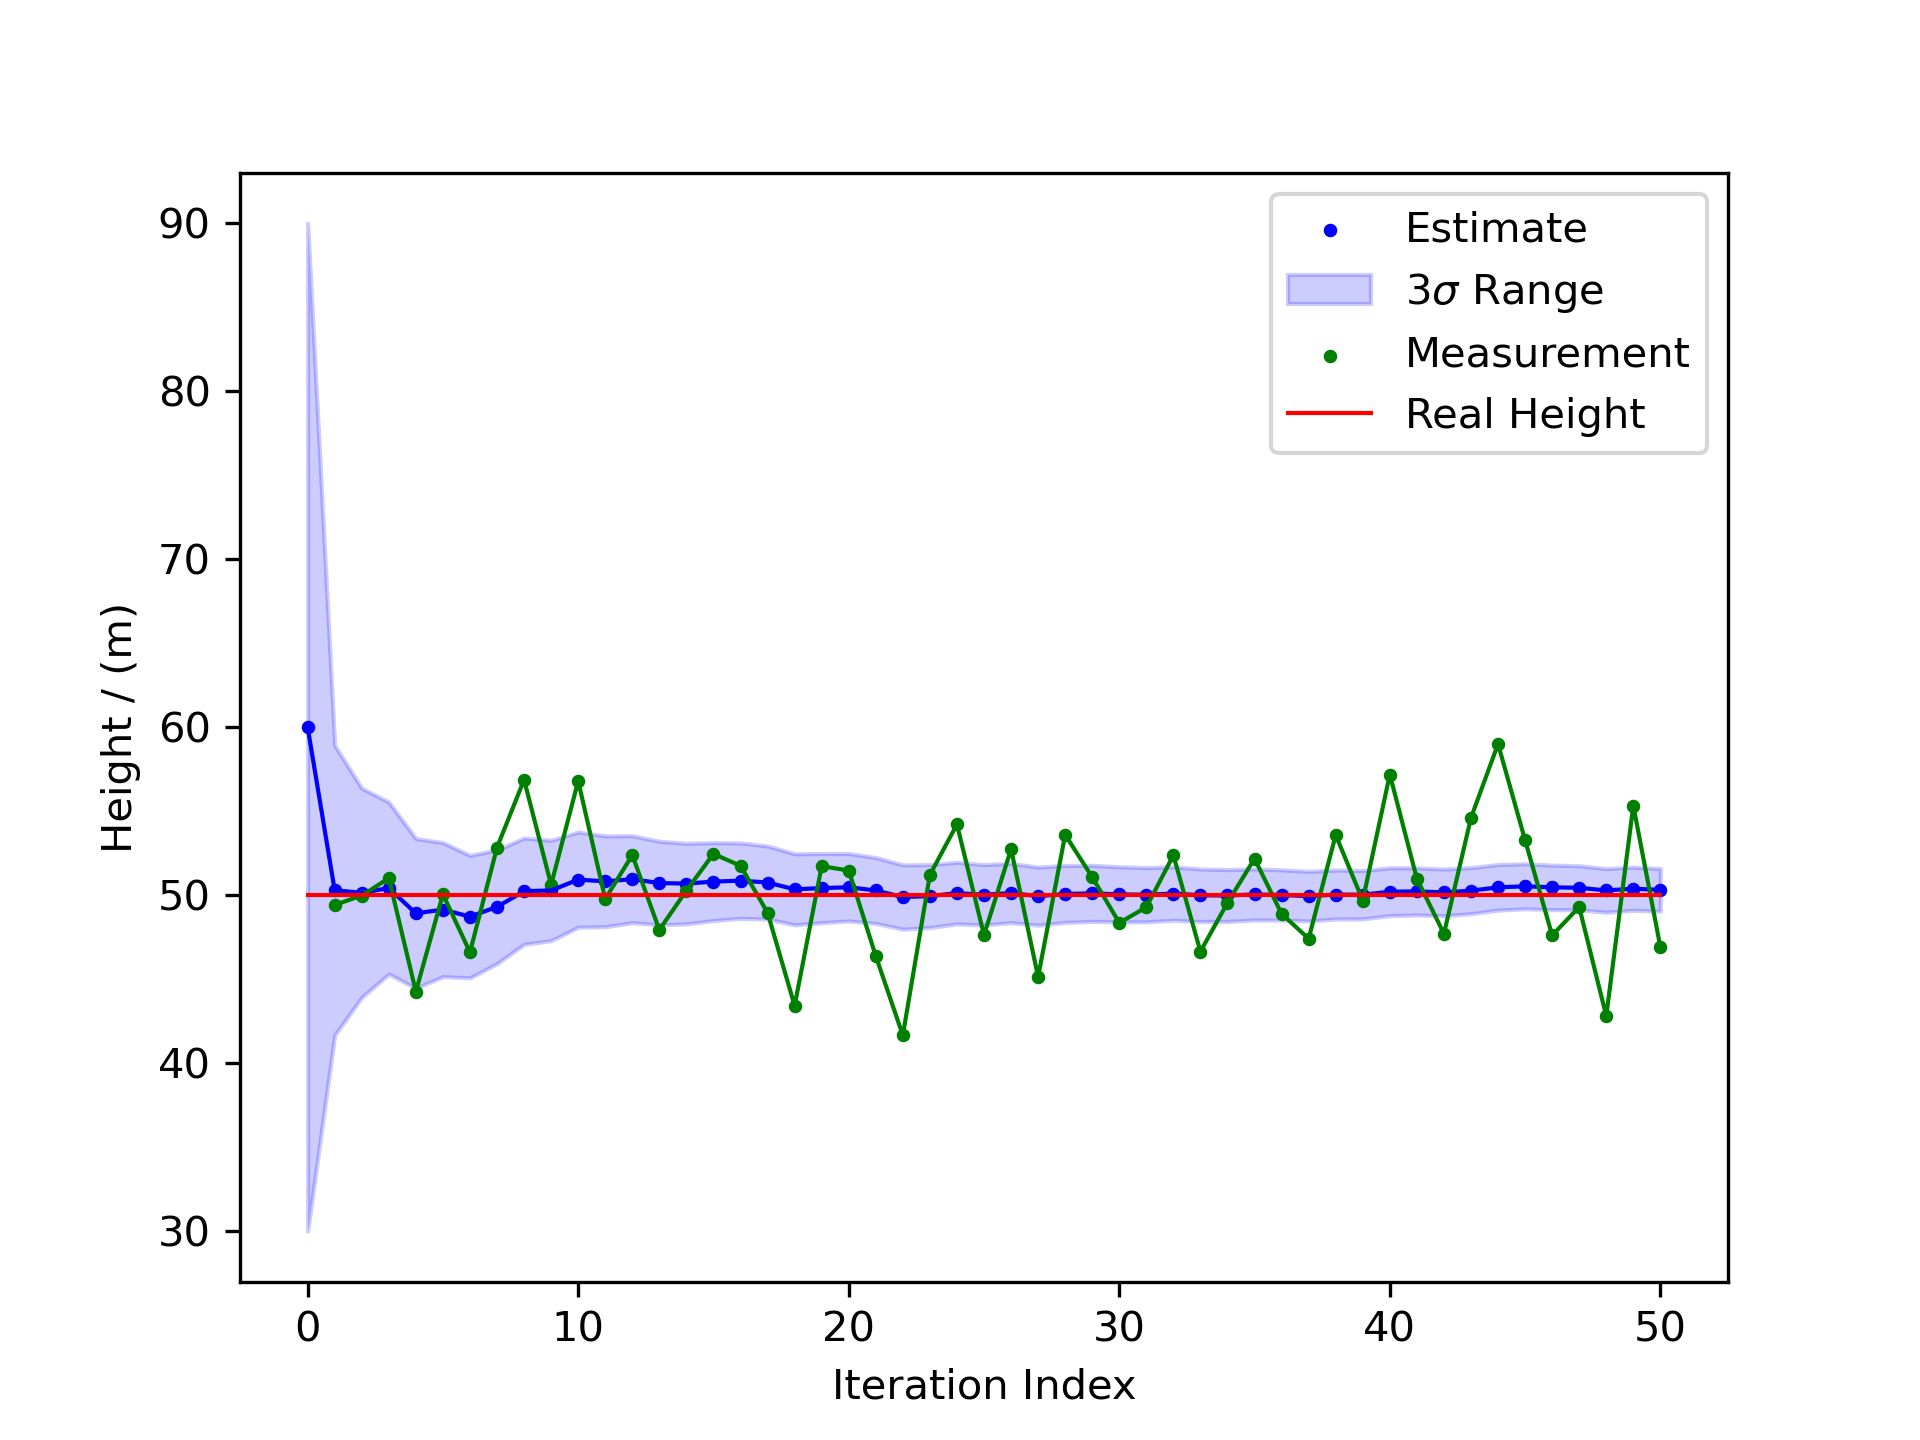
\includegraphics[width=0.7\textwidth]{./figures/exp1} 
   \caption{测量楼的高度结果}
   \label{fig:exp1}
\end{figure}

\subsection{匀速运动的载具}

设有一个载具在$x$-$y$平面内做匀速运动, 其运动有:
\begin{equation*}
\begin{aligned}
x &= 0.0 + 1.0 t \\
y & = 0.0 + 1.2 t \\
\dot{x} &= 1.0 \\
\dot{y} &= 1.2
\end{aligned}
\end{equation*}

于是容易得到, 对于其状态量$\bm{x} = (x, y, \dot{x}, \dot{y})^T$有状态转移矩阵:
\begin{equation*}
\bm{F} =    
   \begin{pmatrix} % or pmatrix or bmatrix or Bmatrix or ...
      1.0 & 0.0 & \Delta t & 0.0\\
      0.0 & 1.0 & 0.0 & \Delta t \\
      0.0 & 0.0 & 1.0 & 0.0 \\
      0.0 & 0.0 & 0.0 & 1.0 \\
   \end{pmatrix}
\end{equation*}
且对于该力学模型, 没有过程误差, 即:
\begin{equation*}
\bm{Q} =    
   \begin{pmatrix} % or pmatrix or bmatrix or Bmatrix or ...
      0.0 & 0.0 & 0.0 & 0.0\\
      0.0 & 0.0 & 0.0 & 0.0 \\
      0.0 & 0.0 & 0.0 & 0.0 \\
      0.0 & 0.0 & 0.0 & 0.0 \\
   \end{pmatrix}
\end{equation*}

考察对载具状态的观测, 我们假设我们只可以观测到载具的位置(事实上, 速度信息在实际工程应用中也是容易得到的, 但是这里我们不使用速度信息), 即有观测矩阵:
\begin{equation*}
\bm{H} = 
   \begin{pmatrix} % or pmatrix or bmatrix or Bmatrix or ...
      1.0 & 0.0 & 0.0 & 0.0\\
      0.0 & 1.0 & 0.0 & 0.0 \\
   \end{pmatrix}
\end{equation*}
且假设观测误差有$\sigma_x = 1.0 \ \mathrm{m}$, $\sigma_y = 1.0 \ \mathrm{m}$, 于是观测误差协方差矩阵有:
\begin{equation*}
\bm{R} = 
   \begin{pmatrix} % or pmatrix or bmatrix or Bmatrix or ...
      1.0 & 0.0 \\
      0.0 & 1.0 \\
   \end{pmatrix}
\end{equation*}
假设初始的状态量估计和状态量估计协方差为:
\begin{equation*}
\begin{aligned}
\hat{\bm{x}}_{0,0} &= (2.0, 2.0, 2.0, 2.0)^T \\
\bm{P}_{0,0} &=  
   \begin{pmatrix} % or pmatrix or bmatrix or Bmatrix or ...
      4.0 & 0.0 & 0.0 & 0.0\\
      0.0 & 4.0 & 0.0 & 0.0 \\
      0.0 & 0.0 & 1.0 & 0.0 \\
      0.0 & 0.0 & 0.0 & 1.0 \\
   \end{pmatrix}
\end{aligned}
\end{equation*}
采取观测间隔为$1 \ \mathrm{s}$, 得到结果如图\ref{fig:exp2}所示. 即使没有对速度的观测结果, Kalman滤波对于状态量的修正依旧得到了较为准确的位置和速度值. 这一结果基于我们对于系统动力学模型的充分了解, 在下一算例中我们将展示模型不够精确时的结果. 
\begin{figure}[htbp] %  figure placement: here, top, bottom, or page
   \centering
   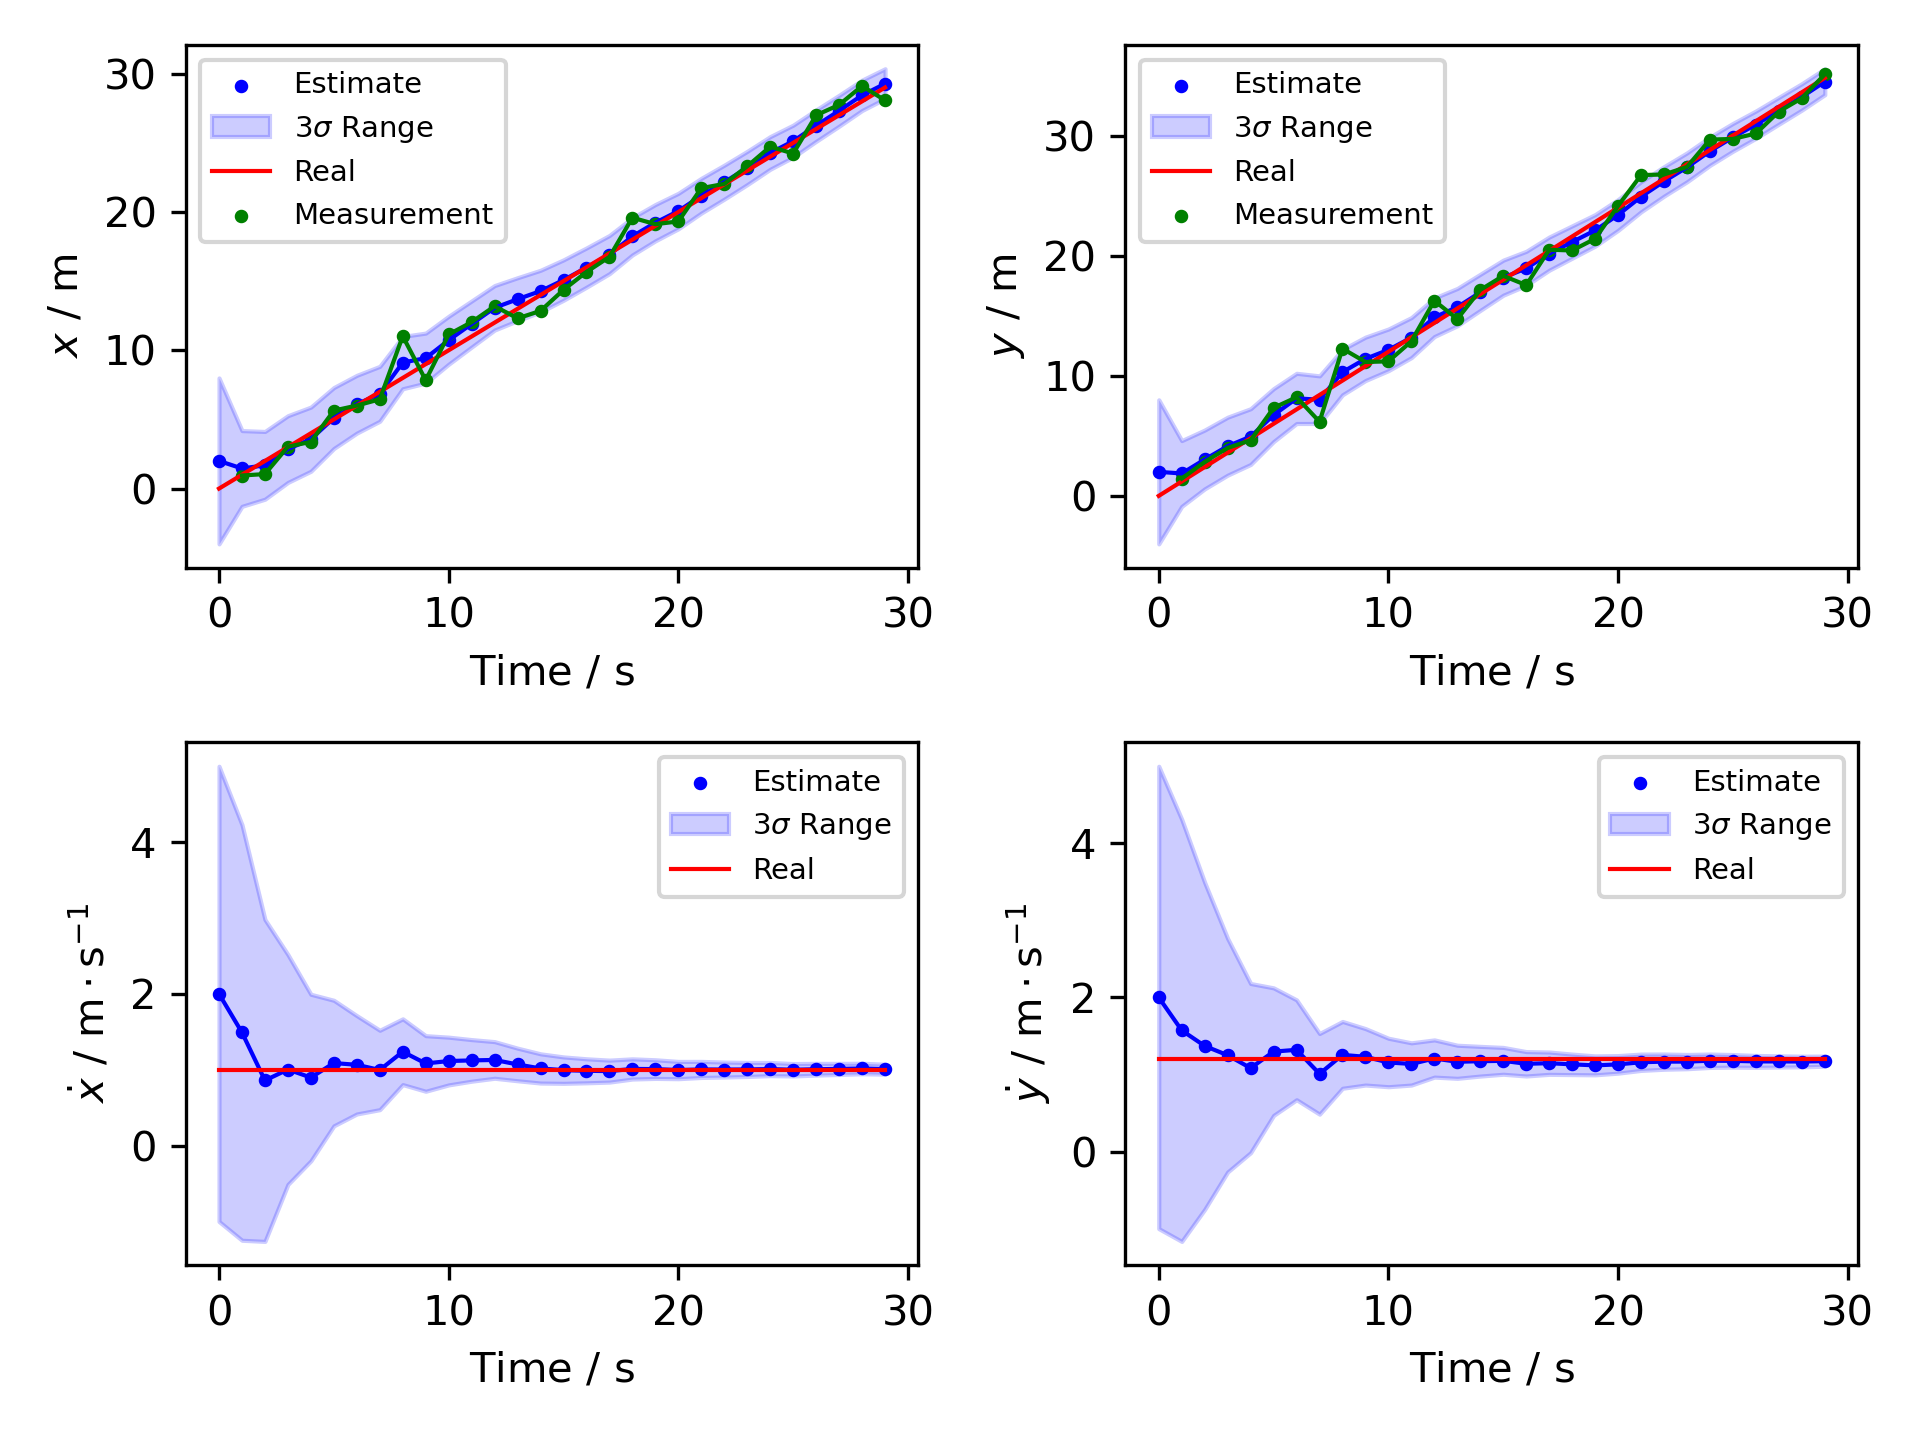
\includegraphics[width=0.7\textwidth]{./figures/exp2} 
   \caption{匀速运动载具观测更新结果}
   \label{fig:exp2}
\end{figure} 

\subsection{做匀加速直线运动的载具}

设有一个载具在$x$-$y$平面内做匀加速直线运动, 且有:
\begin{equation*}
\begin{aligned}
x &= 0.0 + 1.0 t + \frac{1}{2} 0.5 t^2 \\
y & = 0.0 + 1.2 t + \frac{1}{2} 0.3 t^2 \\
\dot{x} &= 1.0 + 0.5 t \\
\dot{y} &= 1.2 + 0.3 t \\
\end{aligned}
\end{equation*}

仿照上例构建数值实验, 参数如表\ref{tab:experimaent_3_parameters_state4}所示. 选取观测间隔为$1 \ \mathrm{s}$, 得到结果如图\ref{fig:exp3_1}所示. 容易看到, 虽然估计结果的协方差在减小, 但是真实值并不在置信区间内. 这是由于所选取的动力学模型(状态转移矩阵)不合适所引起的, 被称为\textbf{Lag Error}. 于是想到通过修改过程噪声矩阵来尝试修正这一问题. 考虑匀加速直线运动, 最主要的误差来自于加速度对速度的影响, 于是简单对过程噪声矩阵进行估计:
\begin{equation*}
\bm{Q} =    
   \begin{pmatrix} % or pmatrix or bmatrix or Bmatrix or ...
      0.0 & 0.0 & 0.0 & 0.0\\
      0.0 & 0.0 & 0.0 & 0.0 \\
      0.0 & 0.0 & 0.25 & 0.0 \\
      0.0 & 0.0 & 0.0 & 0.09 \\
   \end{pmatrix}
\end{equation*}
注意, 这里的估计是很粗略的, 因为实际上过程误差对位置也有影响, 且位置速度的误差并不独立, 即矩阵并非只有对角线元素. 粗略的估计下得到的结果如图\ref{fig:exp3_2}所示. 虽然置信区间受过程误差影响不再收敛, 但是预测结果准确性明显提升. 

当然, 更好的方法是修正动力学模型, 应该将加速度加入载具的状态量中. 在这一例中, 准确的状态转移矩阵写为:
\begin{equation*}
\bm{F} =    
   \begin{pmatrix} % or pmatrix or bmatrix or Bmatrix or ...
      1.0 & 0.0 & \Delta t & 0.0 & \frac{1}{2} \Delta t^2 & 0.0 \\
      0.0 & 1.0 & 0.0 & \Delta t & 0.0 & \frac{1}{2} \Delta t^2 \\
      0.0 & 0.0 & 1.0 & 0.0 & \Delta t & 0.0 \\
      0.0 & 0.0 & 0.0 & 1.0 & 0.0 & \Delta t \\
      0.0 & 0.0 & 0.0 & 0.0 & 1.0 & 0.0 \\
      0.0 & 0.0 & 0.0 & 0.0 & 0.0 & 1.0 \\
   \end{pmatrix}
\end{equation*}
对应状态量向量$\bm{x} = (x, y, \dot{x}, \dot{y}, \ddot{x}, \ddot{y})^T$. 同样考虑只能观测到位置信息的情况, 于是有输入参数如表\ref{tab:experimaent_3_parameters_state6}所示. 所得结果如图\ref{fig:exp3_3}所示, 结果准确且置信区间收敛. 
\begin{table}[htbp]
\centering
\caption{观测匀加速直线运动的载具数值实验参数表(使用四参数估计)}
\label{tab:experimaent_3_parameters_state4}
\begin{tabular}{cc} 
\hline 			
参数 & 说明  \\  
\hline 
$\bm{F} =    
   \begin{pmatrix} % or pmatrix or bmatrix or Bmatrix or ...
      1.0 & 0.0 & \Delta t & 0.0\\
      0.0 & 1.0 & 0.0 & \Delta t \\
      0.0 & 0.0 & 1.0 & 0.0 \\
      0.0 & 0.0 & 0.0 & 1.0 \\
   \end{pmatrix}$ & 状态转移矩阵 \\ 
$\bm{Q} =    
   \begin{pmatrix} % or pmatrix or bmatrix or Bmatrix or ...
      0.0 & 0.0 & 0.0 & 0.0\\
      0.0 & 0.0 & 0.0 & 0.0 \\
      0.0 & 0.0 & 0.0 & 0.0 \\
      0.0 & 0.0 & 0.0 & 0.0 \\
   \end{pmatrix}$ & 过程误差协方差 \\
$\bm{H} = 
   \begin{pmatrix} % or pmatrix or bmatrix or Bmatrix or ...
      1.0 & 0.0 & 0.0 & 0.0\\
      0.0 & 1.0 & 0.0 & 0.0 \\
   \end{pmatrix}$ & 观测矩阵 \\
$\bm{R} = 
   \begin{pmatrix} % or pmatrix or bmatrix or Bmatrix or ...
      1.0 & 0.0 \\
      0.0 & 1.0 \\
   \end{pmatrix}$ & 观测误差协方差 \\
$\hat{\bm{x}}_{0,0} = (2.0, 2.0, 2.0, 2.0)^T$ & 初始状态量估计 \\
$\bm{P}_{0,0} =  
   \begin{pmatrix} % or pmatrix or bmatrix or Bmatrix or ...
      4.0 & 0.0 & 0.0 & 0.0\\
      0.0 & 4.0 & 0.0 & 0.0 \\
      0.0 & 0.0 & 1.0 & 0.0 \\
      0.0 & 0.0 & 0.0 & 1.0 \\
   \end{pmatrix}$ & 初始状态量协方差 \\
\hline 
\end{tabular}
\end{table}

\begin{figure}[htbp] %  figure placement: here, top, bottom, or page
   \centering
   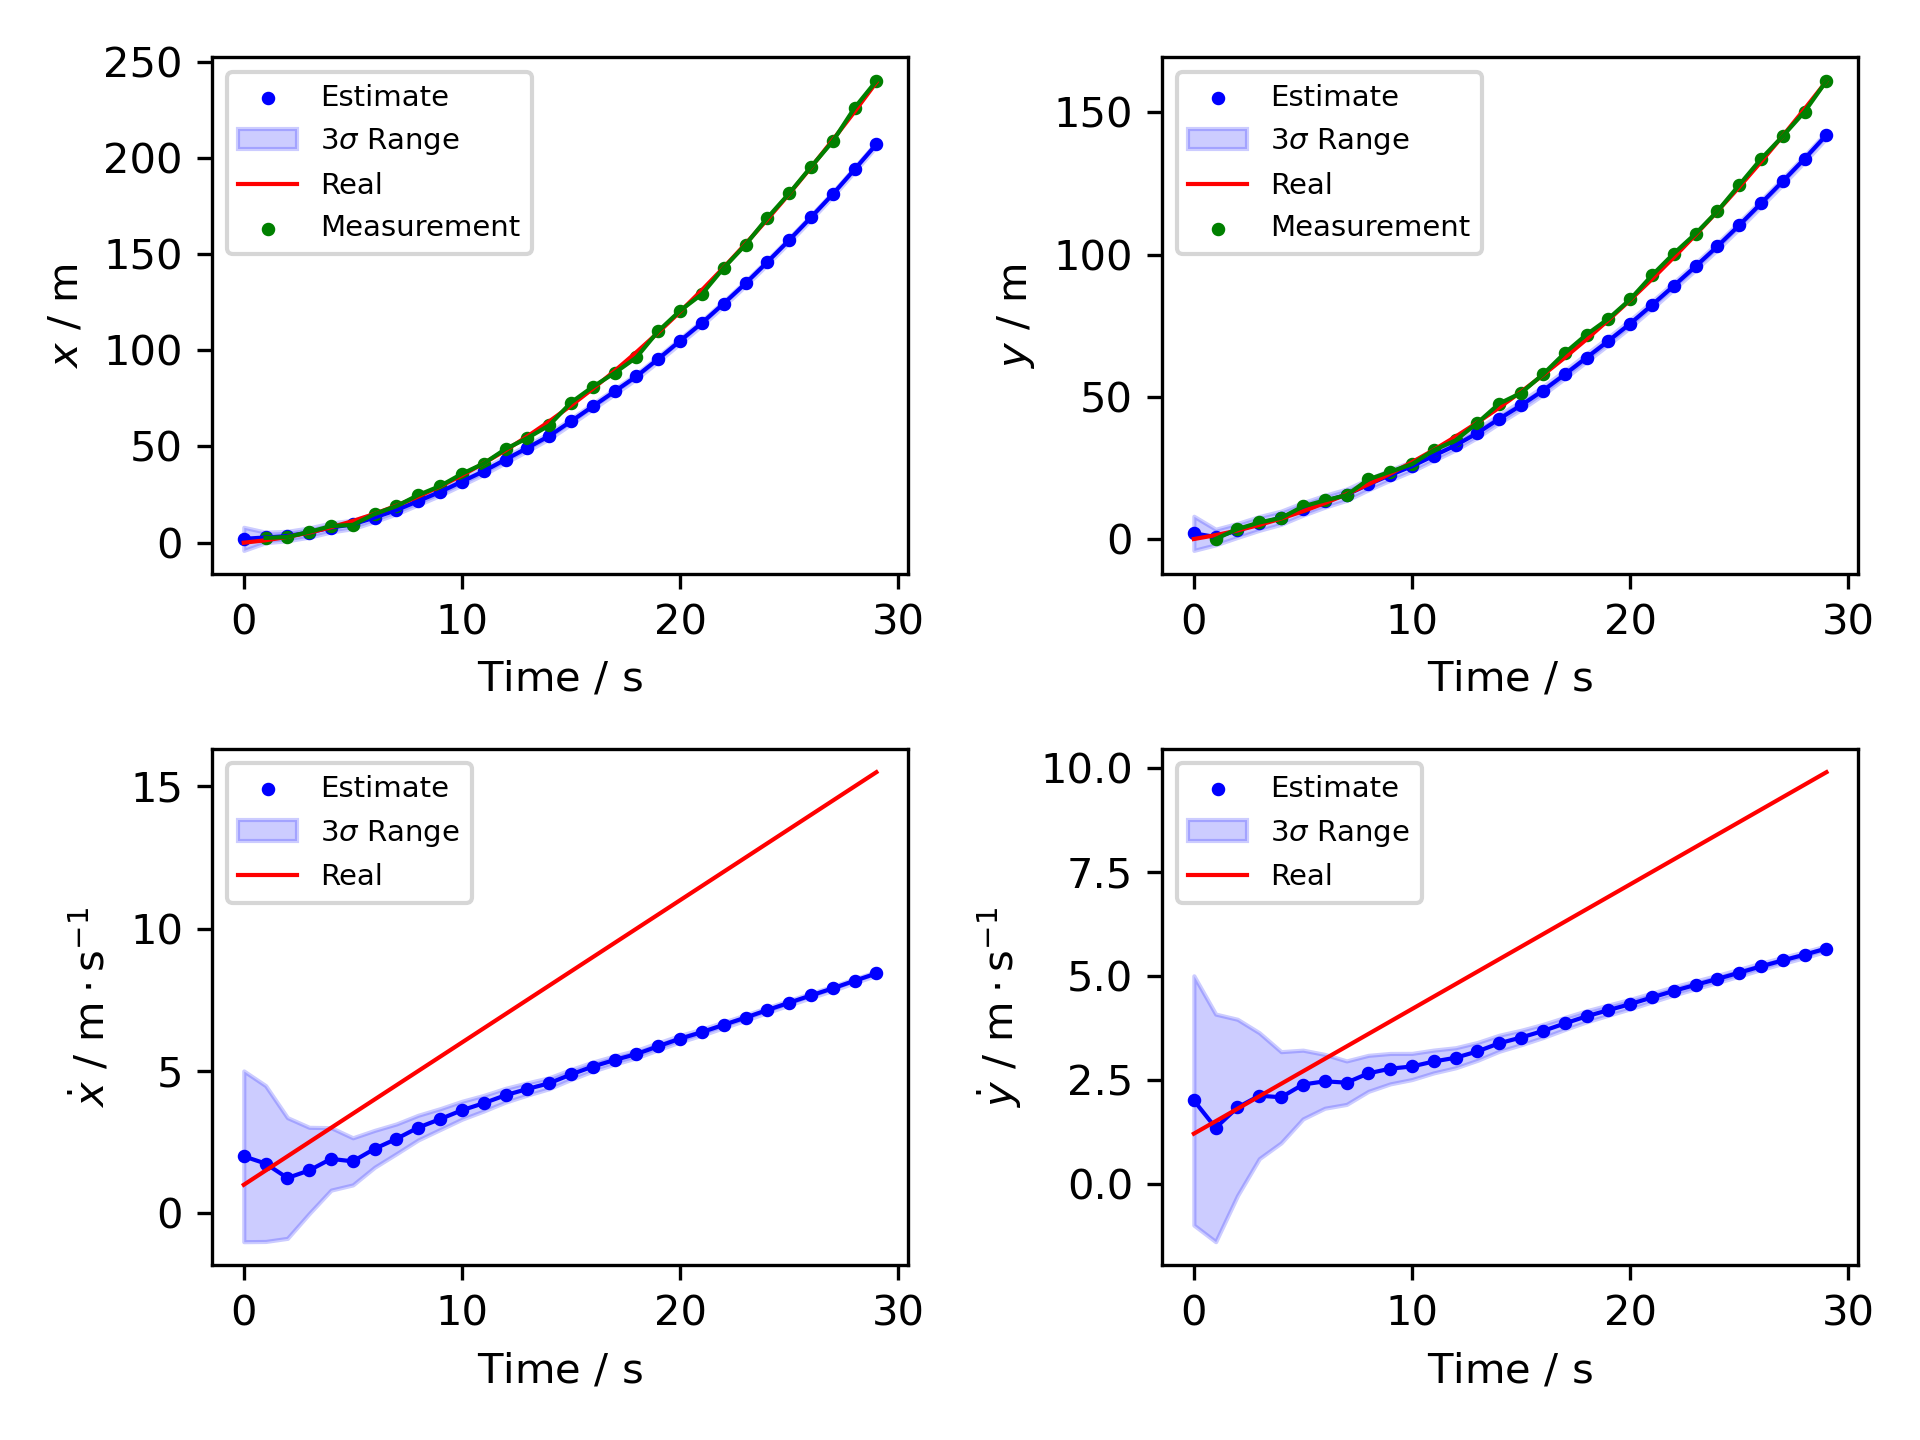
\includegraphics[width=0.7\textwidth]{./figures/exp3_1} 
   \caption{匀加速运动载具观测更新结果(使用四参数估计)}
   \label{fig:exp3_1}
\end{figure} 

\begin{figure}[htbp] %  figure placement: here, top, bottom, or page
   \centering
   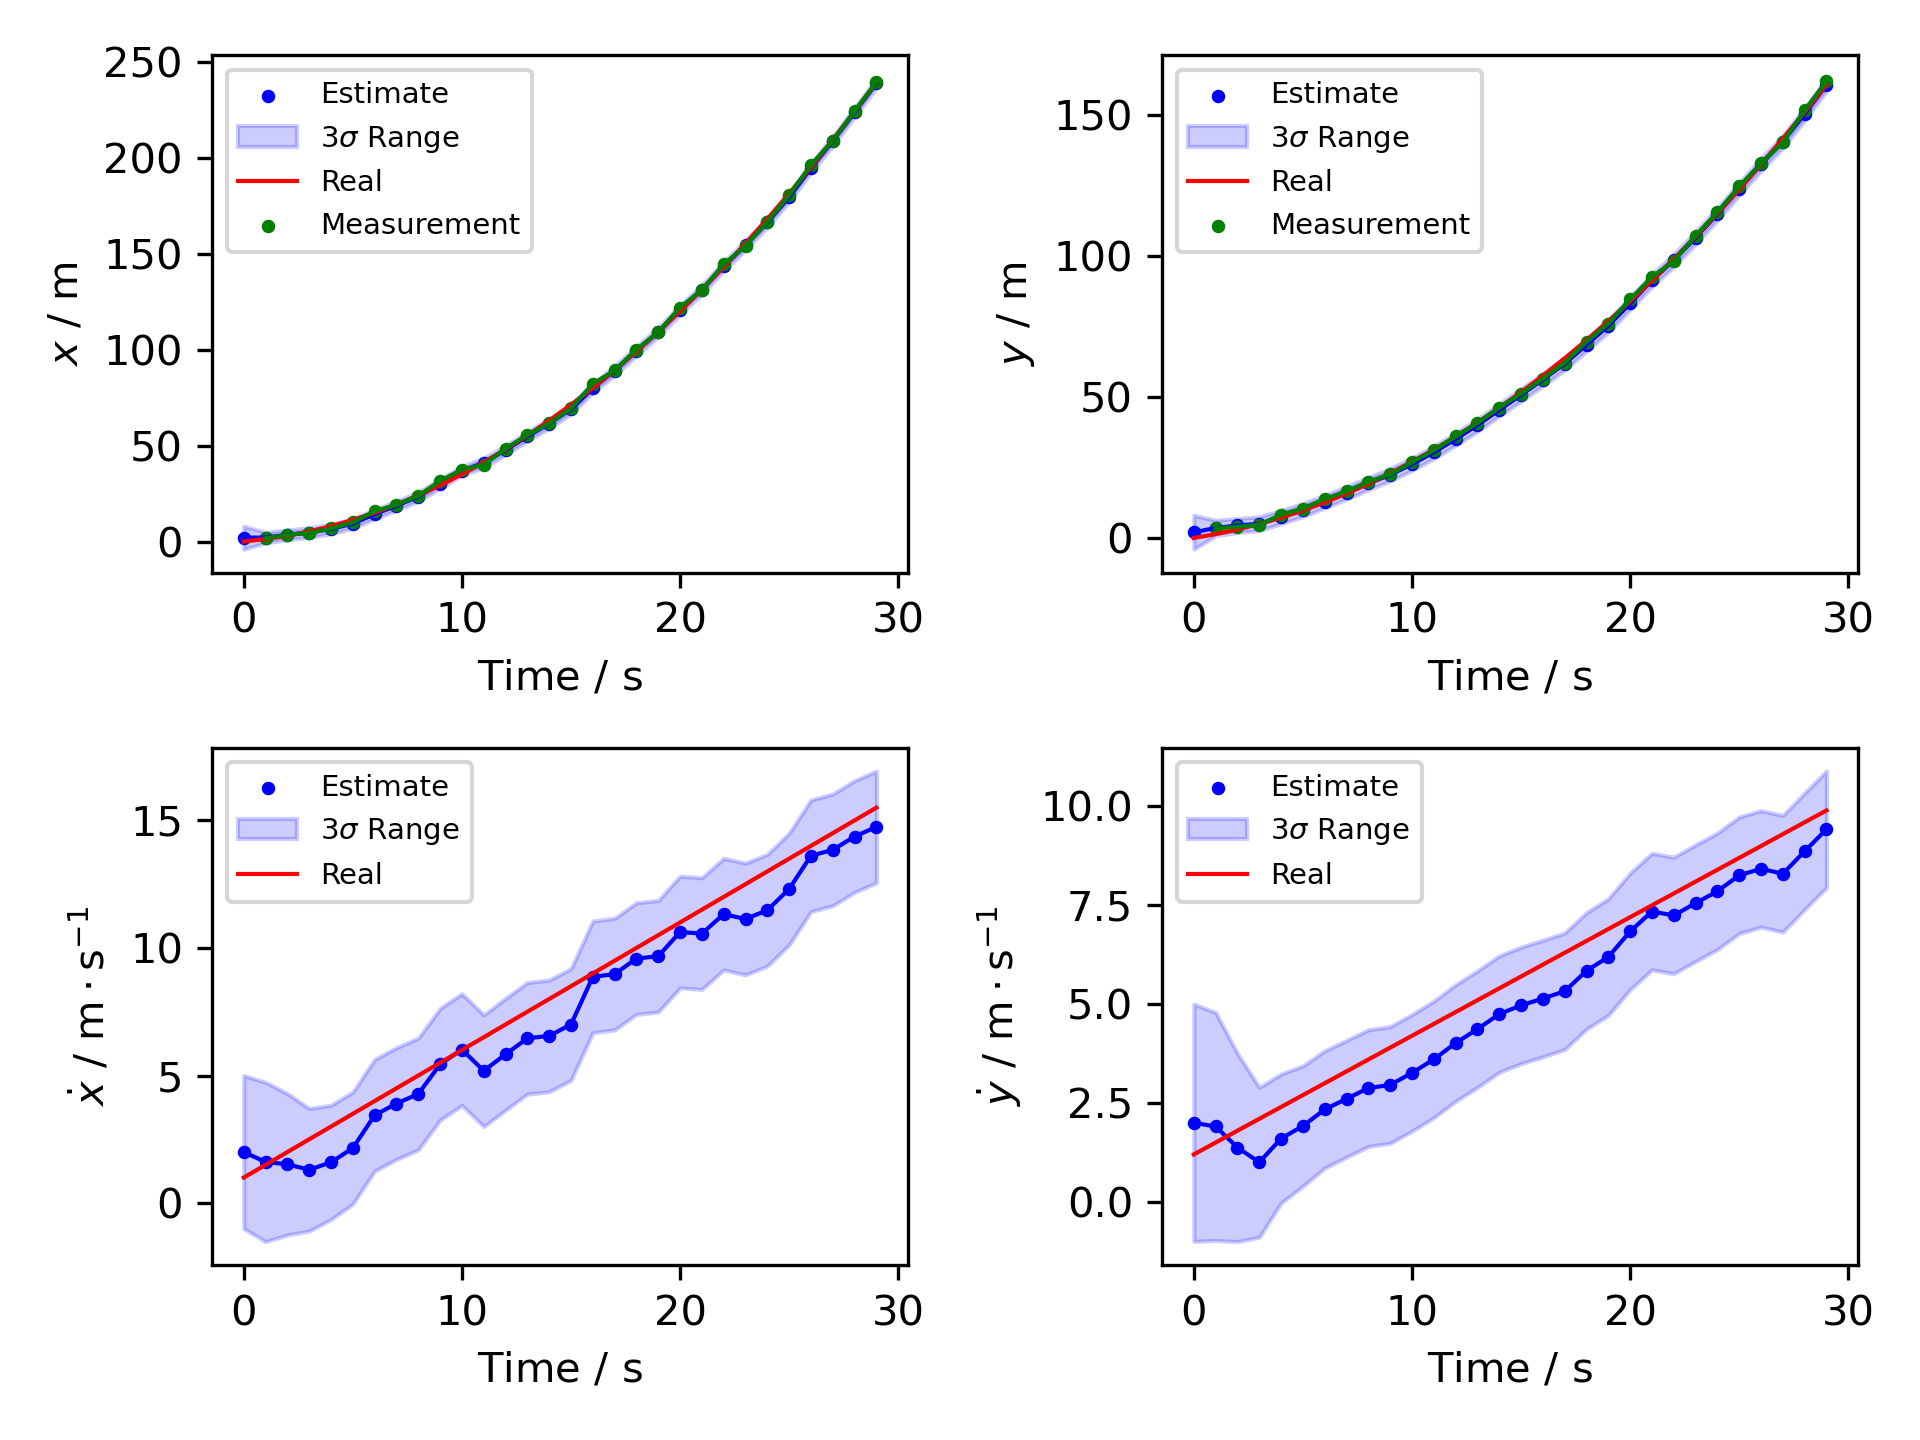
\includegraphics[width=0.7\textwidth]{./figures/exp3_2} 
   \caption{匀加速运动载具观测更新结果(使用四参数估计, 并添加过程噪声)}
   \label{fig:exp3_2}
\end{figure}

\begin{table}[htbp]
\centering
\caption{观测匀加速直线运动的载具数值实验参数表(使用六参数估计)}
\label{tab:experimaent_3_parameters_state6}
\begin{tabular}{cc} 
\hline 			
参数 & 说明  \\  
\hline 
$\bm{F} =    
   \begin{pmatrix} % or pmatrix or bmatrix or Bmatrix or ...
      1.0 & 0.0 & \Delta t & 0.0 & \frac{1}{2} \Delta t^2 & 0.0 \\
      0.0 & 1.0 & 0.0 & \Delta t & 0.0 & \frac{1}{2} \Delta t^2 \\
      0.0 & 0.0 & 1.0 & 0.0 & \Delta t & 0.0 \\
      0.0 & 0.0 & 0.0 & 1.0 & 0.0 & \Delta t \\
      0.0 & 0.0 & 0.0 & 0.0 & 1.0 & 0.0 \\
      0.0 & 0.0 & 0.0 & 0.0 & 0.0 & 1.0 \\
   \end{pmatrix}$ & 状态转移矩阵 \\ 
$\bm{Q} =    
   \begin{pmatrix} % or pmatrix or bmatrix or Bmatrix or ...
      0.0 & 0.0 & 0.0 & 0.0 & 0.0 & 0.0 \\
      0.0 & 0.0 & 0.0 & 0.0 & 0.0 & 0.0 \\
      0.0 & 0.0 & 0.0 & 0.0 & 0.0 & 0.0 \\
      0.0 & 0.0 & 0.0 & 0.0 & 0.0 & 0.0 \\
      0.0 & 0.0 & 0.0 & 0.0 & 0.0 & 0.0 \\
      0.0 & 0.0 & 0.0 & 0.0 & 0.0 & 0.0 \\
   \end{pmatrix}$ & 过程误差协方差 \\
$\bm{H} = 
   \begin{pmatrix} % or pmatrix or bmatrix or Bmatrix or ...
      1.0 & 0.0 & 0.0 & 0.0 & 0.0 & 0.0 \\
      0.0 & 1.0 & 0.0 & 0.0 & 0.0 & 0.0 \\
   \end{pmatrix}$ & 观测矩阵 \\
$\bm{R} = 
   \begin{pmatrix} % or pmatrix or bmatrix or Bmatrix or ...
      1.0 & 0.0 \\
      0.0 & 1.0 \\
   \end{pmatrix}$ & 观测误差协方差 \\
$\hat{\bm{x}}_{0,0} = (2.0, 2.0, 2.0, 2.0, 0.0, 0.0)^T$ & 初始状态量估计 \\
$\bm{P}_{0,0} =  
   \begin{pmatrix} % or pmatrix or bmatrix or Bmatrix or ...
      4.0 & 0.0 & 0.0 & 0.0 & 0.0 & 0.0 \\
      0.0 & 4.0 & 0.0 & 0.0 & 0.0 & 0.0 \\
      0.0 & 0.0 & 1.0 & 0.0 & 0.0 & 0.0 \\
      0.0 & 0.0 & 0.0 & 1.0 & 0.0 & 0.0 \\
      0.0 & 0.0 & 0.0 & 0.0 & 1.0 & 0.0 \\ 
      0.0 & 0.0 & 0.0 & 0.0 & 0.0 & 1.0 \\
   \end{pmatrix}$ & 初始状态量协方差 \\
\hline 
\end{tabular}
\end{table}

\begin{figure}[htbp] %  figure placement: here, top, bottom, or page
   \centering
   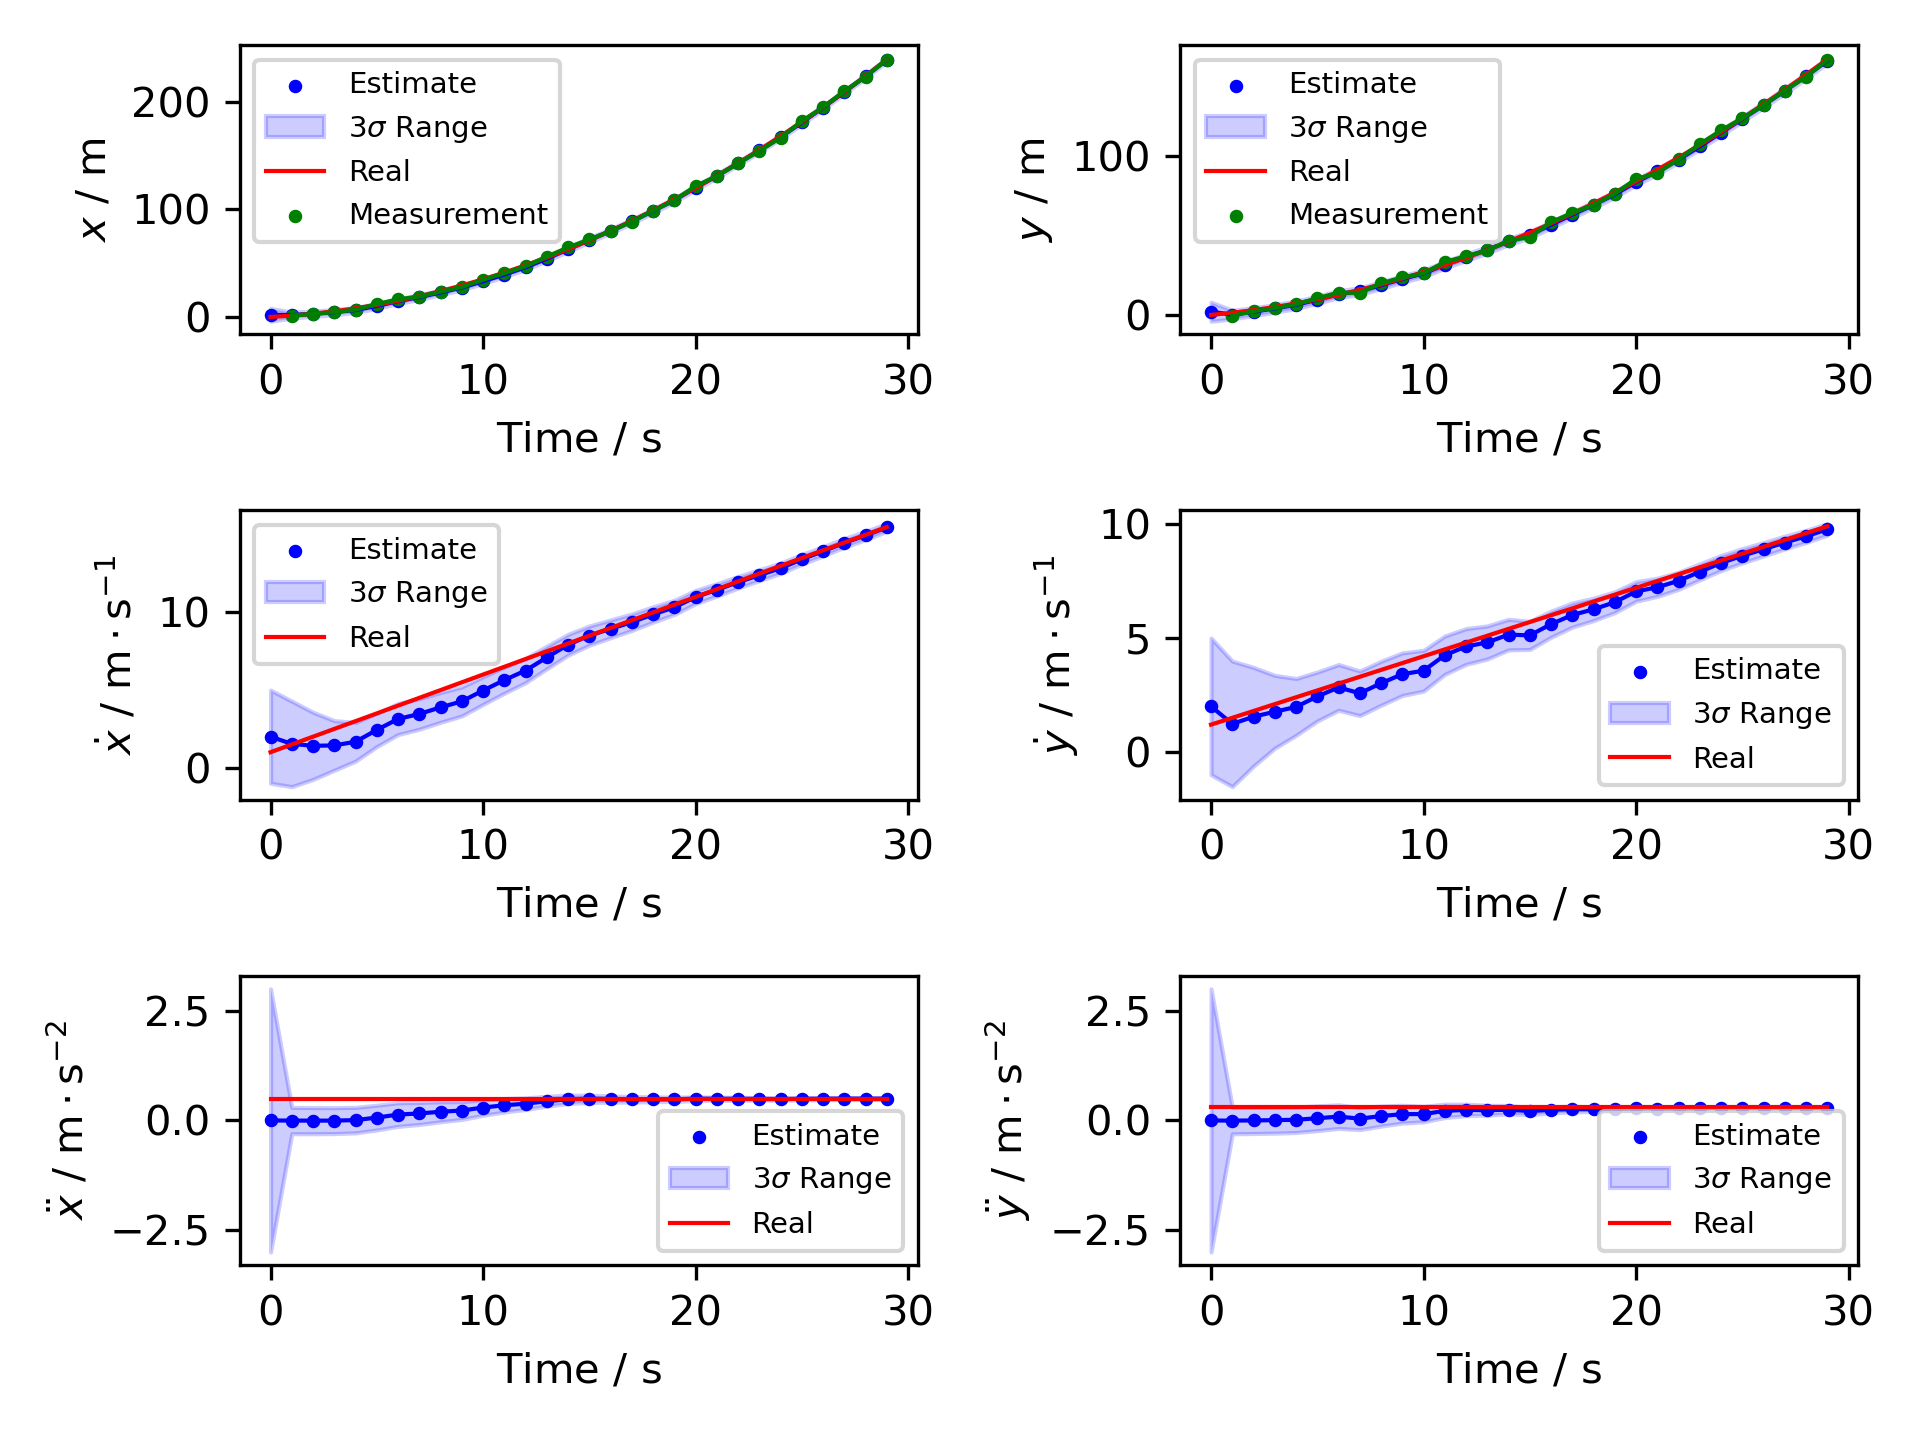
\includegraphics[width=0.7\textwidth]{./figures/exp3_3} 
   \caption{匀加速运动载具观测更新结果(使用六参数估计)}
   \label{fig:exp3_3}
\end{figure}

\section{总结}

本文介绍了Kalman滤波程序的基本原理和实现, 并提供了诸多测试案例供读者学习. 若对代码或案例有任何疑问, 可咨询作者: ajax0514@hotmail.com



\end{document}